\documentclass[12pt]{article}
\usepackage[margin=1cm]{geometry}
\usepackage{polski}
\usepackage[utf8]{inputenc}
\usepackage{siunitx}
\usepackage{amsmath}
\usepackage{graphicx}
\usepackage{multicol}
\usepackage{nopageno}
\usepackage{subcaption}

\newenvironment{Figure}
  {\par\medskip\noindent\minipage{\linewidth}}
  {\endminipage\par\medskip}
  
 \newcommand{\moment}{\si{\kg \times \m^{2}}}

\title{\textbf{Moduł Younga - sprawozdanie}}
\author{Karol Pietruszka\\Konrad Lewandowski}
\date{}

\begin{document}
\noindent
\begin{center}
\begin{tabular}{|l|l|l|l|l|}
\hline
Wydział: EAIIB                                                       & \begin{tabular}[c]{@{}l@{}}Konrad Lewandowski\\ Karol Pietruszka\end{tabular} & 2016          & pt. 9.45        & Zespół: 8 \\ \hline
\begin{tabular}[c]{@{}l@{}}PRACOWNIA\\ FIZYCZNA\\ WFiIS\end{tabular} & \multicolumn{3}{l|}{Temat: Moduł Younga}                                                                    & 11        \\ \hline
\begin{tabular}[c]{@{}l@{}}Data wykonania\\ 7.01.2016\end{tabular}    & \begin{tabular}[c]{@{}l@{}}Data oddania:\\ 11.01.2016\end{tabular}              & Zwrot do pop. & Data zaliczenia & Ocena     \\[10ex] \hline
\end{tabular}
\end{center}
\vspace{2em}

\section{Wstęp}
Celem laboratorium było wyznaczenie modułu Younga dla mosiądzu i stali, na podstawie zależności wydłużenia odcinka drutu, poddanego działaniu siły rozciągającej (zawieszania coraz cięszych odważników).
\section{Dane}
\subsection{Pomiary długości i średnicy drutów poddawanych rozciągnaiu}
\begin{multicols}{2}
Dla drutu stalowego:

Średnica $ \phi_{s} = \frac{0.76 + 0.76 + 0.75 + 0.75}{4} = 0.755\si{\mm}$

Długośc $L_{s} = 1067\si{\mm}$
\columnbreak

Dla drutu mosiężnego

Średnica $ \phi_{m} = \frac{1.15 + 1.16 + 1.17 + 1.17}{4} = 1.162\si{\mm}$

Długośc $L_{m} = 1070\si{\mm}$

\end{multicols}

\subsection{Pomiary wydłużenia drutów poddanych obciążeniu}

M - obciążenie [\si{\kg}]\\\\
W1S - dwukrotność\footnote{Spowodowane dźwignią 1:2 na przyrządzie pomiarowym} wydłużenia drutu stalowego podczas dokładania kolejnych obciążeń [\si{\um}]\\
W2S - dwukrotność wydłużenie drutu stalowego podczas zdejmowania kolejnych obciążeń [\si{\um}]\\
W1M, W2M - Analogiczne wartości dla drutu mosiężnego\\
$W_s = \frac{W1S + W2S}{4}$ - średnia wartość wydłużenia drutu stalowego [\si{\um}]\\
$W_m = \frac{W1M + W2M}{4}$ - średnia wartość wydłużenia drutu mosiężnego [\si{\um}]
\begin{table}[h!]
\centering
\label{my-label}
\begin{tabular}{|l|l|l|l|l|l|l|}
\hline
M & W1S & W2S & W1M & W2M & $W_S$ & $W_M$      \\ \hline
0,982    & 130      & 200      & 610         & 620         & 85             & 307,5           \\ \hline
2,015    & 450      & 480      & 1090        & 1110        & 235            & 550              \\ \hline
2,996    & 700      & 720      & 1720        & 1420        & 355            & 710              \\ \hline
3,985    & 930      & 950      & 1730        & 1740        & 470            & 867,5           \\ \hline
4,996    & 1150     & 1160     & 2010        & 2030        & 585            & 1010             \\ \hline
5,996    & 1360     & 1400     & 2290        & 2290        & 695            & 1140             \\ \hline
7,044    & 1610     & 1660     & 2540        & 2550        & 820            & 1275           \\ \hline
8,012    & 1830     & 1870     & 2780        & 2800        & 925            & 1395           \\ \hline
8,994    & 2060     & 2130     & 3020        & 3030        & 1042,5         & 1512,5          \\ \hline
10,022   & 2270     & 2320     & 3250        & 3290        & 1150           & 1635           \\ \hline
\end{tabular}
\end{table}

\subsection{Wyniki pomiarów}
Proste z poniższych wykresów odzwierciedlają następującą zależność: \\

$\Delta l = aF$ - wydłużenie zależy liniowo od siły rozciągającej ($a$ - współczynnik kierunkowy prostej regresji liniowej). Zgodnie z prawem Hooke'a $a =\frac{l}{ES}$. Rozpisując $\Delta l = a M g$ i podstawiając otrzymujemy:
\begin{equation}
    E = \frac{4lg}{\pi \phi^{2} a}
\end{equation}
Wyniki liczbowe pomiarów:
\begin{table}[ht]
\centering
\begin{tabular}{l|c|c|c|}
\cline{2-4}
                               & Współczynnik kierunkowy [\si{\frac{\um}{\N}}] & Niepewność & Obliczone E [\si{\GPa}] \\ \hline
\multicolumn{1}{|l|}{Stali}  & 116              & 0.000013   & 203.54\\ \hline
\multicolumn{1}{|l|}{Mosiądzu} & 1417              & 0.0000049  & 74.343 \\ \hline
\end{tabular}
\end{table}

\subsection{Niepewności pomiarowe}
$u(\phi) = \frac{0.01}{\sqrt{3}}\si{\mm}$ - na podstawie działki elementarnej śruby mikrometrycznej\\
$u(l) = \frac{1}{\sqrt{3}}\si{\mm}$ - na podstawie działki elementarnej linijki
\\\\
Przy obliczaniu niepewności modułu Younga korzystamy ze standardowego wzoru na propagację niepewności względnej: 

\begin{align}
    \frac{u_{c}(E)}{E} &= \sqrt{ \left( \frac{ \frac{4g}{\pi \cdot d^{2} a}}{ \frac{4lg}{\pi \cdot d^{2} a }} \right)^{2} 
                               + \left( \frac{ \frac{-2 \cdot 4g}{\pi \cdot d^{3} a}}{ \frac{4lg}{\pi \cdot d^{2} a }} \right)^{2} 
                               + \left( \frac{ \frac{-1 \cdot 4g}{\pi \cdot d^{2} a^{2}}}{ \frac{4lg}{\pi \cdot d^{2} a }} \right)^{2} } \\
    \frac{u_{c}(E)}{E} &= \sqrt{ \left(\frac{u(l)}{l}\right)^{2} + \left(-2 \frac{u(d)}{d}\right)^{2} +\left(-1 \frac{u(a)}{a}\right)^{2} } 
\end{align}
\\
\begin{multicols}{2}
Obliczenie niepewnośći dla stali:
\begin{align}
    \frac{u_{c}(E)}{E} &= \sqrt{ (9.3e-4)^{2} + ( 2.6e-2 )^{2} + (1.1e-1)^{2})}\\
    \frac{u_{c}(E)}{E} &= 0.00311\\
    u_{c}(E) &= 0.66\si{\GPa}
\end{align}

Obliczenie niepewnośći pomiarowej dla mosiądzu:
\begin{align}
    \frac{u_{c}(E)}{E} &= \sqrt{ (9.3e-4)^{2} + ( 1.7e-2 )^{2} + (1.1e-3)^{2})}\\
    \frac{u_{c}(E)}{E} &= 0.0011\\
    u_{c}(E) &= 0.082\si{\GPa}
\end{align}
\end{multicols}

\section{Wnioski}
Po porównaniu z wartościami tablicowymi (E mosiądzu $\in (103, 123)$, E stali $\in (190, 210)$), możemy stwierdzić, że przyrząd pomiarowy pozwolił jedynie na poprawne wyznaczenie modułu Younga stali. (gdyż wartość E mosiądzu nie mieści się w tablicowym przedziale), lub badana próbka materiału była wykonana ze stopu innego niż tablicowy mosiądz (inne proporcje miedzi i cynku)

\begin{figure}[b]
  \centering
  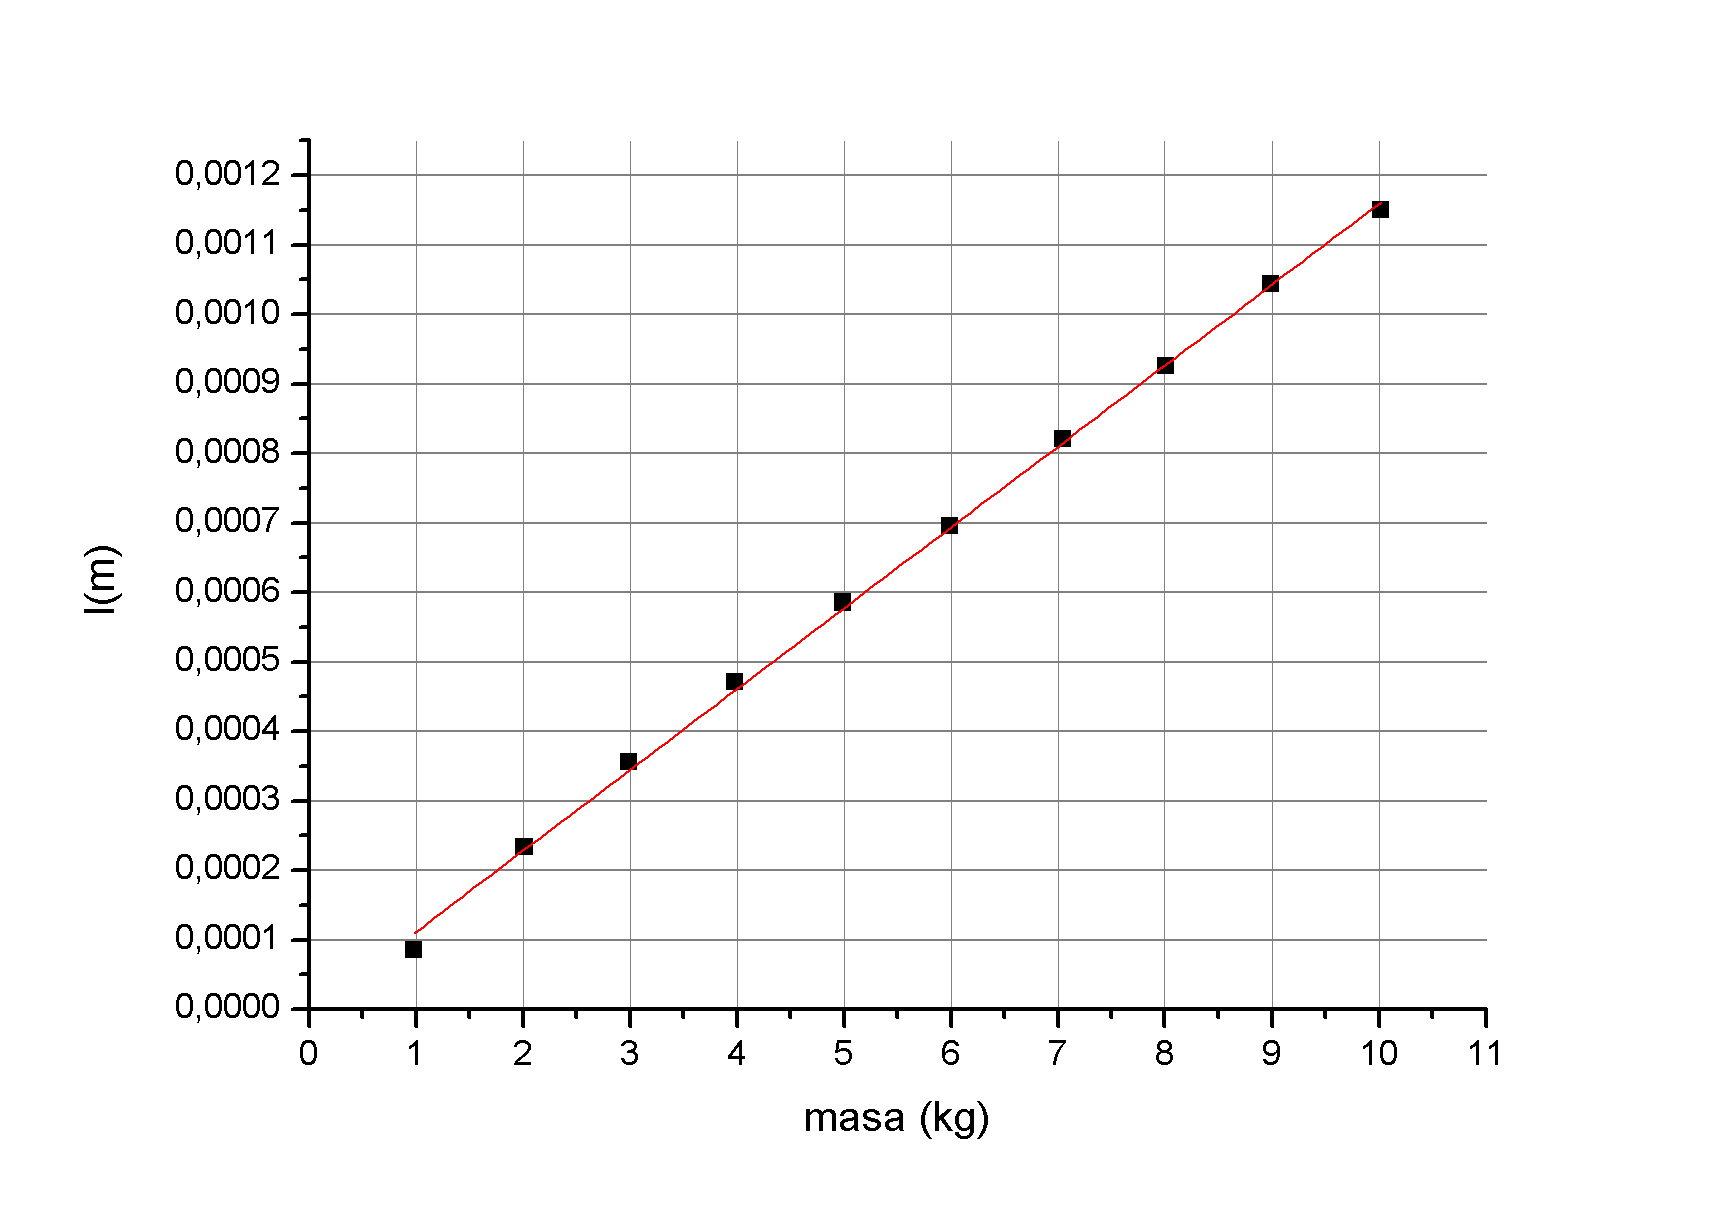
\includegraphics[width=.8\linewidth]{Grap2.jpg}
  \caption{Wyniki pomiarów dla drutu stalowego}
  \centering
  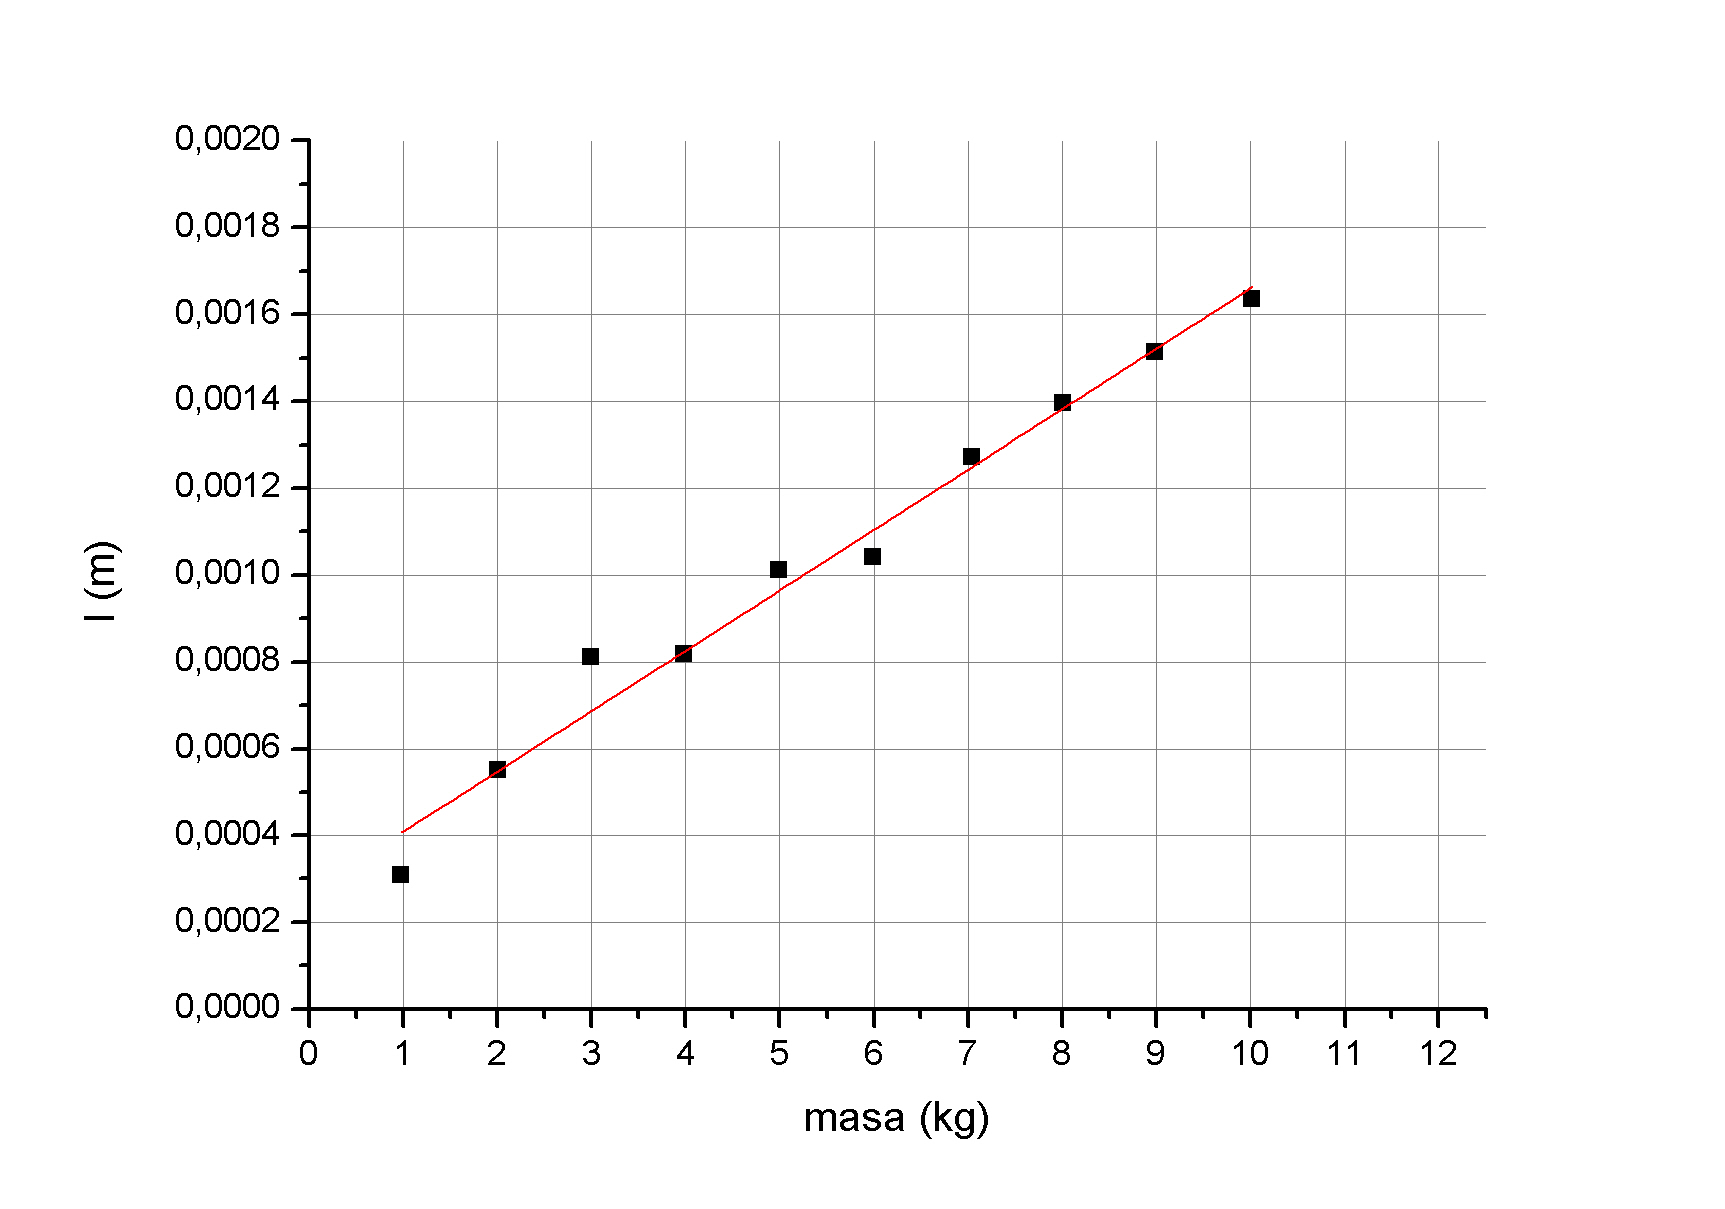
\includegraphics[width=.8\linewidth]{Grap3.jpg}
  \caption{Wyniki pomiarów dla drutu mosiężnego}
\end{figure}


\end{document}
